\chapter{Monitoring layer}\label{G:monitoringLayer}

As already discussed, in order to properly manage a cloud computing environment it is strongly required to use monitoring tools in order to gather information of interest by improving the environment itself or by finding out issues and solving them as fast as possible.

This chapter aims to showcase how the selected monitoring tools can fit in the architecture type that has been proposed. And, how they can be used. This means, preparing the environment to support Collectd (i.e.: monitoring and gathering) and Graphite (i.e.: storing and presenting) tools.

Moreover, to point out that such tools are helpful to demonstrate that LiveMediaStreamer framework could be deployed as the core of a real-time media production platform (see chapter \ref{H:platformDeploymentAndDemonstrations}).

So, to remark that the fact of creating small and reusable containers is the main goal of this chapter and, of course, the goal of this platform architecture to prototype. And, thanks to the selected monitoring tools, which are lightweight and ease configuration flexibility, this issue might be properly solved.

Then, a proposal of the monitoring architecture in a more detailed description (regarding figure \ref{F:MLAP}) is shown in figure \ref{F:maex}.

\begin{figure}[htb]
\begin{center}
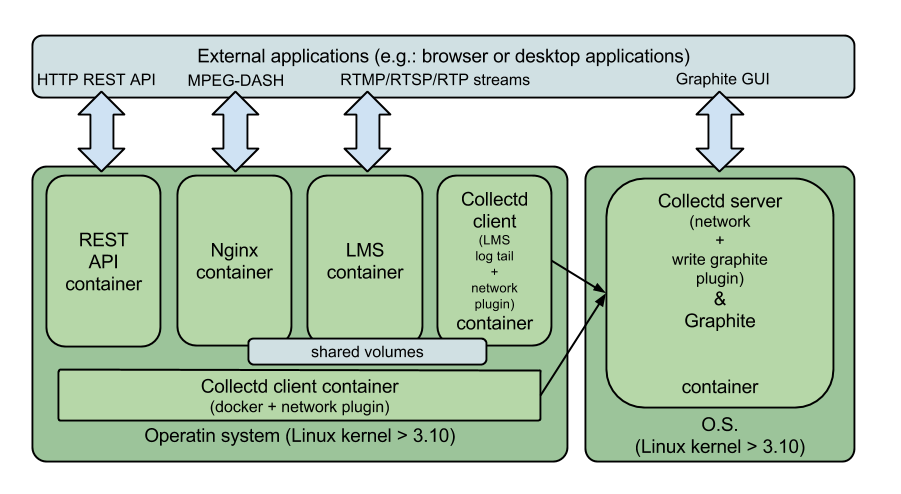
\includegraphics[width=0.9\textwidth]{./images/monitArchProp.png}
\caption{Detailed monitoring architecture}
\label{F:maex}
\end{center}
\end{figure}

Figure \ref{F:maex} showcases the relationship between different containers and the whole Collectd+Graphite deployment. Following sections are explaining it:

\section{Monitoring containers}

This section is based on how Collectd can be configured and deployed in order to monitor and properly gather metrics of interest.

\subsection{From O.S. point of view}

The fact of using Collectd means a wide community behind, which probably have already developed required functionalities (i.e.: plugins). And this is the case: in order to monitor each of the containers that a host O.S. might have it can be solved by configuring already existing plugins for Collectd from Docker community. 

The selected plugin is using the stats API introduced since Docker 1.5 version. And, concretely, the reported container's stats are:
 
\begin{itemize}
\item Network bandwidth
\item Memory usage
\item CPU usage
\item Block IO
\end{itemize}

The pluguin is called "docker-collectd-pluguin" and can be found in \href{https://github.com/lebauce/docker-collectd-plugin}{GitHub} (--REFERENCE--).

Therefore, the O.S. system requires having a basic collectd daemon running and to be configured in order to send gathered metrics to a centralized collectd server (as proposed in figure \ref{F:maex}).

So, from O.S. point of view, next example of this specific Collectd's plugins configuration showcases how to load and configure such plugins:

\begin{verbatim}

TypesDB "/usr/share/collectd/docker-collectd-plugin/dockerplugin.db"
LoadPlugin python

<Plugin python>
  ModulePath "/usr/share/collectd/docker-collectd-plugin"
  Import "dockerplugin"

  <Module dockerplugin>
    BaseURL "unix://var/run/docker.sock"
    Timeout 3
  </Module>
</Plugin>

LoadPlugin network
<Plugin network>
  Server "graphite-host-address" "graphite-host-port"
  ReportStats true
</Plugin>

\end{verbatim}

Previous Collectd configuration file sets the python (i.e.: docker-collectd-plugin) plugin as an input from the O.S. Docker API daemon and the network plugin as an output to the Collectd server.

\subsection{From container point of view}

From a container point of view and by following the premise to build containers as reusable as possible what is proposed to implement is a container that has the goal to gather the logged stats from an LMS container. This, as shown in figure \ref{F:maex}, implies sharing a Docker volume (as introduced in previous chapter \ref{D:virtualization}) from LMS container to the Collectd client which is using the tail plugin as an input. Moreover, in order to send specific logged metrics to the Collectd server container it is also using the network plugin as done in previous Collectd client configuration.




\section{Showcasing monitoring}

container amb graphite + collectd server